\documentclass{standalone}
\usepackage{tikz}
\usetikzlibrary{positioning}
\begin{document}
    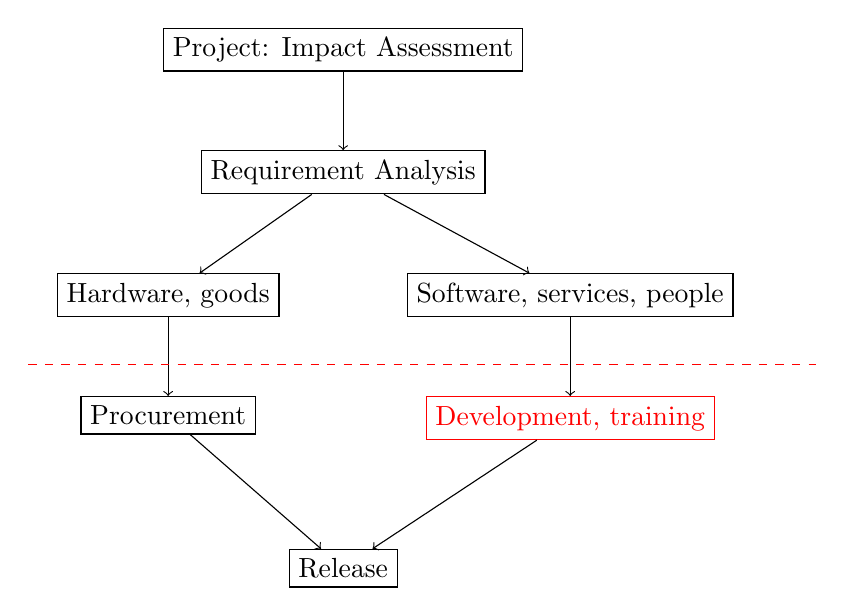
\begin{tikzpicture}
        \tikzset{every node/.style={draw, minimum height=2ex,node distance=1cm and -1cm}}
        \node (pj) {Project: Impact Assessment};
        \node[below=of pj] (a) {Requirement Analysis};
        \node[below left=of a] (h) {Hardware, goods};
        \node[below right=of a] (s) {Software, services, people};
        \node[below=of h] (pc) {Procurement};
        \node[below=of s, color=red] (dt) {Development, training};
        \node[below=4.5cm of a] (re) {Release};
        \draw[->] (pj) -- (a);
        \draw[->] (a) -- (h);
        \draw[->] (a) -- (s);
        \draw[->] (h) -- (pc);
        \draw[->] (s) -- (dt);
        \draw[->] (dt) -- (re);
        \draw[->] (pc) -- (re);
        \draw[dashed, color=red] (-4,-4) -- (6,-4);
    \end{tikzpicture}
\end{document}